\chapter{Th\'eorie des circuits AC} \label{subsec:ac_circuit_theory}

\section{Introduction au courant alternatif} \label{subsec:intro_ac}
Le \emph{courant alternatif} (souvent not\'e \textbf{AC} pour \emph{Alternating Current}) est un type de courant \'electrique dont l’intensit\'e et la direction varient p\'eriodiquement au cours du temps. Contrairement au courant continu (DC), où les \'electrons circulent toujours dans le m\^eme sens, le courant alternatif change de sens à intervalles r\'eguliers, g\'en\'eralement selon une forme sinuso\"idale.\par
Il est g\'en\'eralement repr\'esent\'e pas une onde sinuso\"idale~:
\[
    u(t) = U_{max} \cdot \sin(\omega t + \phi)
\]
o\`u~:
\begin{itemize}
    \item $u(t)$ est la tension instantan\'ee en fonction du temps $t$,
    \item $U_{max}$ est l'amplitude maximale de la tension,
    \item $\omega$ est la pulsation angulaire (en radians par seconde), reli\'ee à la fr\'equence $f$ par la relation $\omega = 2\pi f$,
    \item $\phi$ est la phase initiale (en radians), qui d\'etermine le d\'ecalage de l'onde par rapport au temps $t = 0$.
\end{itemize}

\subsection{La phase}
La \emph{phase} d'une onde sinuso\"idale d\'efinit son \emph{d\'ecalage temporel} par rapport à une r\'ef\'erence. Elle est exprim\'ee en radians (ou en degr\'es) et indique \`a quel point l'onde commence dans son cycle au temps $t = 0$.\par

\begin{figure}[h!]
    \newcounter{angle}
    \setcounter{angle}{220}
    \begin{tikzpicture}
    \draw[thick,-stealth,black] (-3,0)--(4,0) coordinate (A) node[below] {$x$};
    \draw[thick,-stealth,black] (0,-3)--(0,3) node[left] {$y$}; % y axis
    \draw[black,thin] (0,0) circle (2.5cm);
    \node[black,below] at (2.7,0) {1};
    \node[black,above] at (0.2,-3.2) {1};
    \draw (1,0) arc (0:\theangle:1) node at ($(\theangle/2:0.7)$) {$\phi$};
    \draw[dashed, blue] (\theangle:2.5cm) -- (\theangle:2.5cm |- 0,0) node[sloped, rotate=180, yshift=8pt, midway] {$\sin \phi$}; % vertical line
    \draw[ultra thick,red,rotate=\theangle] (0,0) -- (2.5,0) coordinate (B);
    \foreach \x in {0,30,...,360} {\filldraw[black] (\x:2.5cm) circle(1pt);};
    \foreach \x/\xtext in {
            30/\frac{\pi}{6},
            60/\frac{\pi}{3},
            120/\frac{2\pi}{3},
            150/\frac{5\pi}{6},
            210/\frac{7\pi}{6},
            240/\frac{4\pi}{3},
            300/\frac{5\pi}{3},
            330/\frac{11\pi}{6}
            }
        \draw (\x:2.8cm) node {\tiny $\xtext$};
    \foreach \x/\xtext in {
            90/\frac{\pi}{2}}
            \draw (\x:2.7cm) node[xshift=4pt] {\tiny $\xtext$};
    \foreach \x/\xtext in {
            270/\frac{3\pi}{2}}
            \draw (\x:2.7cm) node[xshift=-5pt] {\tiny $\xtext$};
    \foreach \x/\xtext in {
            180/\pi,
            360/2\pi}
            \draw (\x:2.7cm) node[yshift=4pt] {\tiny $\xtext$};

    \begin{scope}
    \begin{axis}[
        thick,
        y=2.5cm,
        axis lines=center,
        xmin=0, xmax=360,
        ymin=-1, ymax=1,
        anchor=origin, at=(A),
        xshift=3ex,
        enlarge y limits,
        enlarge x limits=upper,
        samples=90,
        xtick={0,30,...,360},
    xticklabels={0,
        $\frac{\pi}{6}$,
        $\frac{\pi}{3}$,
        $\frac{\pi}{2}$,
        $\frac{2\pi}{3}$,
        $\frac{5\pi}{6}$,
        $\pi$,
        $\frac{7\pi}{6}$,
        $\frac{4\pi}{3}$,
        $\frac{3\pi}{2}$,
        $\frac{5\pi}{3}$,
        $\frac{11\pi}{6}$,
        $2\pi$
        },
        tick label style={font=\tiny},
        ]
        \addplot[domain=0:\theangle,ultra thick, no markers,blue] {sin(x)} coordinate (C);
        \addplot[domain=\theangle-1:\theangle,ultra thick, no markers,blue] {sin(x)-sin(x)} coordinate (K);
    \end{axis}
    \draw [dashed,red, thick] (B) -- (C);
    \draw [dashed,blue, thick] (C) -- (K);
    \end{scope}
    \tkzDrawPoints(B);
    \end{tikzpicture}
    \label{fig:phase}
    \caption{Repr\'esentation de la phase $\phi$ d'une onde sinuso\"idale.}
\end{figure}

\subsection{Valeur efficace (RMS)}
La valeur efficace (ou RMS, \emph{Root Mean Square}) d'une tension ou d'un courant alternatif est une mesure de la valeur moyenne de la puissance dissip\'ee par le courant.
Pour une onde sinuso\"idale, la valeur efficace de tension et de courant sont donn\'ees par~:
\[
U_{\text{eff}} = \frac{U_{\text{max}}}{\sqrt{2}}, \quad I_{\text{eff}} = \frac{I_{\text{max}}}{\sqrt{2}}
\]
\begin{Note}{\textbf{D'où vient le $\sqrt{2}$ ?}}\\
La formule g\'en\'erale de la valeur efficace est~:
\[
U_{\text{eff}} = \sqrt{\frac{1}{T_2 - T_1} \int_{T_1}^{T_2} [u(t)]^2 \, dt}
\]
avec \( u(t) = U_{\text{max}}\sin(\omega t) \). On obtient alors~:
\[
U_{\text{eff}} = U_{\text{max}} \sqrt{\frac{1}{T_2 - T_1} \int_{T_1}^{T_2} \sin^2(\omega t)\, dt}
\]
En utilisant l'identit\'e trigonom\'etrique $\sin^2(x) = \frac{1 - \cos(2x)}{2}$, on peut \'ecrire~:
\[
\int_{T_1}^{T_2} \sin^2(\omega t)\, dt = \frac{1}{2}(T_2 - T_1)
\]
puisque l’int\'egrale du terme $\cos(2\omega t)$ sur une p\'eriode compl\`ete est nulle.
Ainsi~:
\[
U_{\text{eff}} = U_{\text{max}} \sqrt{\frac{1}{T_2 - T_1} \cdot \frac{T_2 - T_1}{2}} = \frac{U_{\text{max}}}{\sqrt{2}}
\]
\end{Note}
Pour une onde carr\'ee, la valeur efficace est \'egale à l'amplitude maximale~:
\[U_{\text{eff}} = U_{\text{max}}, \quad I_{\text{eff}} = I_{\text{max}}\]
Pour une onde triangulaire, la valeur efficace est donn\'ee par~:
\[U_{\text{eff}} = \frac{U_{\text{max}}}{\sqrt{3}}, \quad I_{\text{eff}} = \frac{I_{\text{max}}}{\sqrt{3}}\]


\subsection{Puissance en AC}
La puissance dans un circuit en courant alternatif d\'epend non seulement de la tension et du courant, mais aussi du d\'ephasage $\phi$ entre eux.
La tension et le courant peuvent \^etre exprim\'es sous forme sinuso\"idale~:
\[
u(t) = U_{\text{max}} \sin(\omega t), \quad i(t) = I_{\text{max}} \sin(\omega t - \phi)
\]
La puissance instantan\'ee vaut alors~:
\[
p(t) = u(t) \cdot i(t) = U_{\text{max}} I_{\text{max}} \sin(\omega t)\sin(\omega t - \phi)
\]
En utilisant l'identit\'e trigonom\'etrique $\sin A \sin B = \tfrac{1}{2}[\cos(A - B) - \cos(A + B)]$, on obtient~:
\[
p(t) = \frac{U_{\text{max}} I_{\text{max}}}{2} [\cos(\phi) - \cos(2\omega t - \phi)]
\]
La puissance instantan\'ee est donc constitu\'ee d’un terme constant et d’un terme variable à la fr\'equence double.

\begin{Note}{\textbf{Puissance moyenne (active)}}\\
Le terme oscillant $\cos(2\omega t - \phi)$ a une moyenne nulle sur une p\'eriode complète.
La puissance moyenne (ou puissance active) est donc~:
\[
P = \frac{U_{\text{max}} I_{\text{max}}}{2} \cos(\phi)
\]
En exprimant les grandeurs en valeurs efficaces~:
\[
U_{\text{eff}} = \frac{U_{\text{max}}}{\sqrt{2}}, \quad I_{\text{eff}} = \frac{I_{\text{max}}}{\sqrt{2}}
\]
on obtient la relation fondamentale~:
\[
\boxed{P = U_{\text{eff}} \cdot I_{\text{eff}} \cdot \cos(\phi)}
\]
où~:
\begin{itemize}
    \item $P$ est la puissance active (en watts, W),
    \item $U_{\text{eff}}$ est la tension efficace (en volts, V),
    \item $I_{\text{eff}}$ est le courant efficace (en ampères, A),
    \item $\phi$ est le d\'ephasage entre la tension et le courant.
\end{itemize}
\end{Note}

\subsubsection*{Les diff\'erentes puissances en r\'egime alternatif}
On distingue trois formes de puissance~:
\begin{itemize}
    \item \textbf{Puissance apparente}~:
    \[
    S = U_{\text{eff}} I_{\text{eff}} \quad [\text{VA}]
    \]
    Elle repr\'esente la puissance totale fournie au circuit.

    \item \textbf{Puissance active}~:
    \[
    P = U_{\text{eff}} I_{\text{eff}} \cos(\phi) \quad [\text{W}]
    \]
    Elle correspond à la puissance r\'eellement consomm\'ee ou convertie en travail ou chaleur.

    \item \textbf{Puissance r\'eactive}~:
    \[
    Q = U_{\text{eff}} I_{\text{eff}} \sin(\phi) \quad [\text{var}]
    \]
    Elle repr\'esente l’\'energie \'echang\'ee p\'eriodiquement entre les champs \'electrique et magn\'etique des composants r\'eactifs (bobines et condensateurs).
\end{itemize}

Ces trois puissances sont li\'ees par la relation~:
\[
S^2 = P^2 + Q^2
\]
et peuvent \^etre repr\'esent\'ees sous forme d’un \textbf{triangle des puissances}.
Le \emph{facteur de puissance}, not\'e $\cos(\phi)$, indique la part de puissance r\'eellement utilis\'ee par le circuit~:
\[
\text{Facteur de puissance} = \frac{P}{S} = \cos(\phi)
\]
Un facteur de puissance proche de \(1\) signifie un usage efficace de l’\'energie \'electrique, tandis qu’un facteur faible traduit une forte composante r\'eactive.
\begin{figure}[h!]
\centering
\begin{tikzpicture}
  \begin{axis}[
    axis lines=middle,
    xlabel={$P$ (W)},
    ylabel={$Q$ (var)},
    xmin=0, xmax=3.8,
    ymin=0, ymax=2.8,
    grid=both,
    width=9cm, height=6cm,
    axis equal image,
    xtick=\empty, ytick=\empty,
    enlargelimits=false,
    axis line style={thick,-latex},
    every axis y label/.style={
        at={(ticklabel cs:0.5)},rotate=90,anchor=near ticklabel,
    },
    every axis x label/.style={
        at={(ticklabel cs:0.5)},anchor=near ticklabel,
    },
  ]
  \coordinate (O) at (axis cs:0,0);
  \coordinate (A) at (axis cs:3,0);   % P
  \coordinate (B) at (axis cs:3,2);   % Q
  \draw[thick, blue] (O) -- node[below, yshift=-2pt] {$P$} (A);
  \draw[thick, red] (A) -- node[right, xshift=2pt] {$Q$} (B);
  \draw[thick, black] (O) -- node[above, rotate=35] {$S=\sqrt{P^2+Q^2}$} (B);
  \draw pic["$\phi$", draw=black, angle radius=8mm, angle eccentricity=1.2] {angle = A--O--B};
  \node at (axis cs:1.5,0.5) {\small $\cos\phi = \dfrac{P}{S}$};
  \end{axis}
\end{tikzpicture}
\caption{Triangle des puissances en r\'egime alternatif~: relation entre $P$, $Q$ et $S$.}
\label{fig:triangle_puissances}
\end{figure}

\section{Circuits RLC} \label{subsec:rlc_circuits}

\subsection{Comportement des composants en AC}

\subsubsection{R\'esistance (R)}
Une r\'esistance dans un circuit en courant alternatif se comporte de la m\^eme manière qu'en courant continu \Cref{subsec:resistors}. Elle ob\'eit à la loi d'Ohm~:
\[
u(t) = R \cdot i(t)
\]
La tension et le courant sont en phase \Cref{fig:R_phase}, atteignant leurs valeurs maximales simultan\'ement. L'imp\'edance est purement r\'eelle~:
\[
Z_R = R
\]
\begin{figure}[h!]
    \centering
    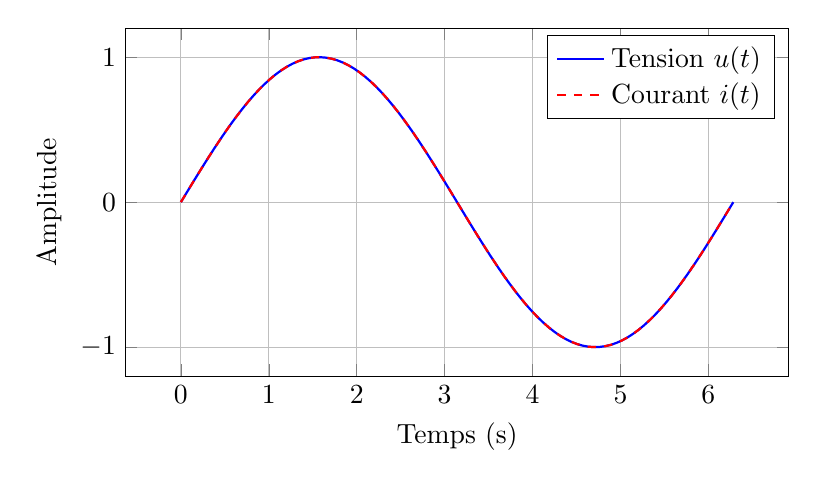
\begin{tikzpicture}
        \begin{axis}[
            xlabel={Temps (s)},
            ylabel={Amplitude},
            grid=both,
            width=10cm,
            height=6cm,
            legend style={at={(0.98,0.98)},anchor=north east},
        ]
        \addplot[domain=0:2*pi,samples=100,blue,thick]{sin(deg(x))};
        \addlegendentry{Tension $u(t)$}
        \addplot[domain=0:2*pi,samples=100,red,dashed,thick]{sin(deg(x))};
        \addlegendentry{Courant $i(t)$}
        \end{axis}
    \end{tikzpicture}
    \caption{R\'esistance~: tension et courant en phase.}
    \label{fig:R_phase}
\end{figure}

\subsubsection{Inductance (L)}
